\begin{figure*}[thb!]
  \centering
  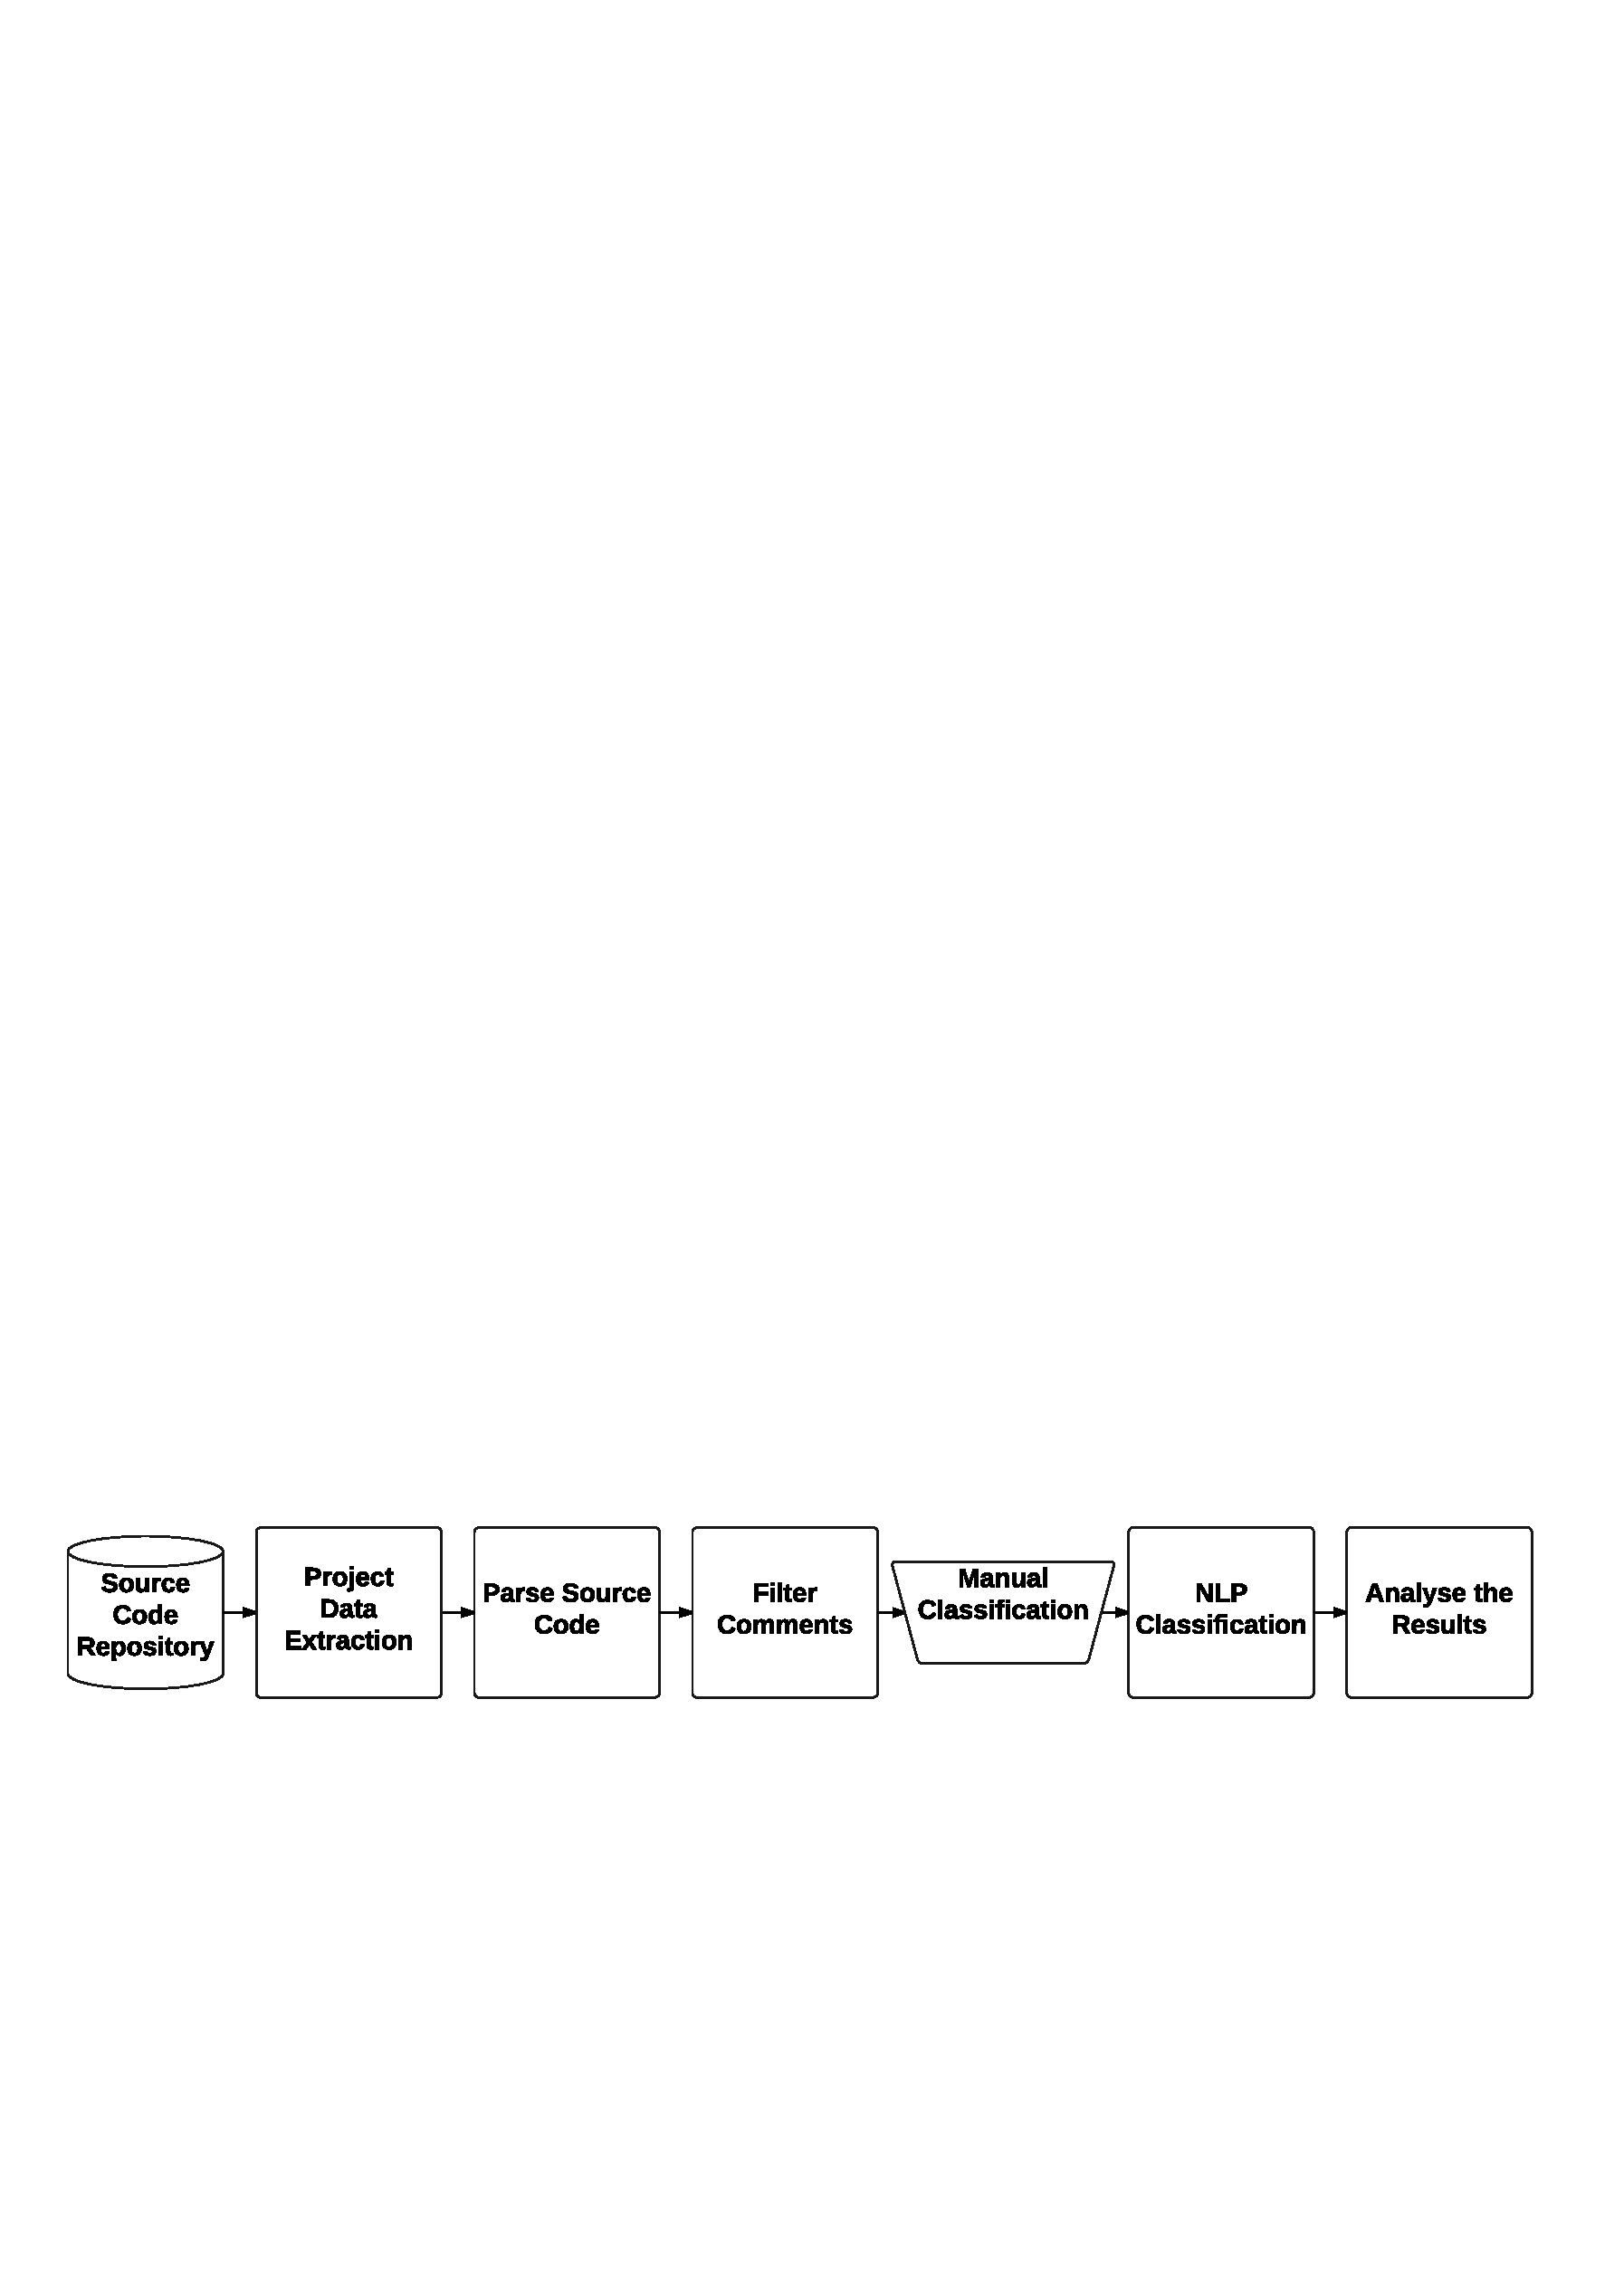
\includegraphics[width=1\textwidth]{figures/approach.pdf}
  \caption{Approach overview}
  \label{fig:approach}
  \vspace{-4mm}
\end{figure*}

The main goal of our study is to automatically identify \SATD through source code comments. To do that, we first extract the comments from ten open source projects. Second, we apply five filtering heuristics to remove comments that are irrelevant for the identification of \SATD  (e.g., license comments, commented source code and Javadoc comments). After that, we manually classify the remaining comments into the different types of \SATD (i.e., design debt, requirement debt, defect debt, documentation debt and test debt). Lastly, we use these comments as training data for the Stanford NLP Classifier and use the trained model to detect \SATD from source code comments. Figure~\ref{fig:approach} shows an overview of our approach, and the following subsections detail each step.

\subsection{Project Data Extraction} % (fold)
\label{sub:data_extraction}

To perform our study, we need to analyze the source code comments of software projects. Therefore, we extract the source code of ten open source projects, namely Ant, Apache Jmeter, ArgoUML, Columba, EMF, Hibernate, JEdit, JFreeChart, JRuby and SQuirrel SQL. We selected these projects since they belong to different application domains, are well commented, vary in size, and in the number of contributors. 

Table~\ref{tab:project_details} provides details about each of the projects used in our study. The columns of Table~\ref{tab:project_details} present the release used, followed by the number of classes, the total source lines of code (SLOC), the number of contributors, the number of extracted comments, the number of comments analyzed after applying our filtering heuristics, the number of comments that were classified as \SATD, the percentage of these comments that represent design debt, the percentage of \SATD comments classified as requirement debt and finally the percentage of all other types of debt (i.e., defect, documentation and test debt). 

Since there are many different definitions for the SLOC metric we clarify that, in our study, a source line of code contains at least one valid character, which is not a blank space or a source code comment. In addition, we only use the Java files to calculate the SLOC, and to do so, we use the SLOCCount tool~\cite{wheeler2004:home}. 

The number of contributors was extracted from OpenHub, an on-line community and public directory that offers analytics, search services and tools for open source software \cite{Openhub:home}. It is important to note that the number of comments shown for each project does not represent the number of commented lines, but rather the number of individual line, block, and Javadoc comments. In total, we obtained 259,229 comments, found in 16,249 Java classes. The size of the selected projects varies between 81,307 and 228,191 SLOC, and the number of contributors of these projects ranges from 9 to 326. 


\begin{table*}[thb!]
    \begin{center}
    \caption{Details of Studied Projects}
    \label{tab:project_details}
    \vspace{-5mm}
            \begin{tabular}{l| c c r c || c c c || c c c}
            \toprule
            
            \textbf{\thead{Project}}   & \textbf{\thead{Release}}  & \textbf{\thead{\# of classes}}   & \textbf{\thead{SLOC}} & \textbf{\thead{\# of \\contributors}}  & \textbf{\thead{\# of \\comments}}   & \textbf{\thead{\# of \\comments \\after filtering}} & \textbf{\thead{\# of \\TD \\comments}} & \textbf{\thead{\% of \\Design \\Debt}} & \textbf{\thead{\% of \\Requirement \\Debt}} & \textbf{\thead{\% of \\Other \\Debts}}\\ 
            \midrule 
            \textbf{Ant}            & 1.7.0    & 1,475 & 115,881 & 74  & 21,587 &   4,137 &    131 &  72.51  & 09.92  & 17.55 \\
            \textbf{ArgoUML}        & 0.34     & 2,609 & 176,839 & 87  & 67,716 &   9,548 &  1,413 &  56.68  & 29.08  & 14.22 \\
            \textbf{Columba}        & 1.4      & 1,711 & 100,200 & 9   & 33,895 &   6,478 &    204 &  61.76  & 21.07  & 17.15 \\
            \textbf{EMF}            & 2.4.1    & 1,458 & 228,191 & 30  & 25,229 &   4,401 &    104 &  75.00  & 15.38  & 09.61 \\
            \textbf{Hibernate}      & 3.3.2 GA & 1,356 & 173,467 & 226 & 11,630 &   2,968 &    472 &  75.21  & 13.55  & 11.22 \\
            \textbf{JEdit}          & 4.2      &   800 &  88,583 & 57  & 16,991 &  10,322 &    256 &  76.56  & 05.46  & 17.96 \\
            \textbf{JFreeChart}     & 1.0.19   & 1,065 & 132,296 & 19  & 23,474 &   4,423 &    209 &  88.03  & 07.17  & 04.78 \\
            \textbf{Jmeter}         & 2.10     & 1,181 &  81,307 & 33  & 20,084 &   8,162 &    374 &  84.49  & 05.61  & 09.89 \\
            \textbf{JRuby}          & 1.4.0    & 1,486 & 150,060 & 328 & 11,149 &   4,897 &    622 &  55.14  & 17.68  & 27.17 \\ 
            \textbf{SQuirrel}       & 3.0.3    & 3,108 & 215,234 & 46  & 27,474 &   7,230 &    286 &  73.07  & 17.48  & 09.44 \\ 
            \bottomrule             
        \end{tabular}
    \end{center}
\end{table*}


% subsection data_extraction (end)
\subsection{Parse Source Code} % (fold)
\label{sub:parse_source_code}

After obtaining the source code of all projects, we extract the comments from the source code. We use JDeodorant \cite{Tsantalis2008CSMR}, an open-source Eclipse plug-in, to parse the source code and extract the code comments. JDeodorant uses the Eclipse AST parser to create an Abstract Syntax Tree (AST) of each Java file. The AST contains detailed information about the source code comments such as: their type (i.e., Block, Single-line, or Javadoc), their location (e.g., inside a method, or a type declaration), and the lines where they start and end. 

Due to these features, we adapted JDeodorant to extract the aforementioned information about source code comments and store it in a relational database to facilitate the processing of the data.

% subsection parse_source_code (end)
\subsection{Filter Comments} % (fold)
\label{sub:filter_comments}

Source code comments can be used for different purposes in a project, such as giving context, documenting, expressing thoughts, opinions and authorship, and in some cases, disabling source code from the program. Comments are used freely by developers and with limited formalities, if any at all. This informal environment allows developers to bring to light opinions, insights and even confessions (e.g., self-admitted technical debt). 

As shown in prior work by Potdar and Shihab \cite{Potdar2014ICSME}, part of these comments can be identified as self-admitted technical debt, but they are not the majority of cases. With that in mind, we develop and apply 5 filtering heuristics to narrow down the comments eliminating the ones that are less likely to be classified as self-admitted technical debt.

To do so, we developed a Java based tool that reads from the database the data obtained by parsing the source code. Next, it executes the filtering heuristics and stores the results back in the database. The retrieved data contains information like the line number that a class/comment begins/ends and the type, considering the Java syntax, of the comment (i.e., Block, Single-line or Javadoc). With this information we process the filtering heuristics as described next.

License comments are not very likely to contain self-admitted technical debt, and are commonly added before the declaration of the class. We create a heuristic that removes comments that are placed before the class declaration. Since we know the line number that the class was declared we can easily check for comments that are placed before that line and remove them. In order to decrease the chances of removing a self-admitted technical debt comment while executing this filter we calibrated this heuristic to not remove comments containing one of task-reserved words (i.e., ``todo'', ``fixme'', or ``xxx'') ~\cite{Storey2008ICSE}.

Long comments that are created using multiple \emph{single-line} comments instead of a \emph{Block} comment can hinder the understanding of the message considering the case that the reader (i.e., human or machine) analyzes each one of these comments independently. To solve that problem, we create a heuristic that searches for consecutive Single-line comments and groups them as one comment.
%We identify consecutive comments by subtracting the line number of both comments. For example, Single-line comment A is placed in line number 100 and Single-line comment B is placed in line 101. The subtraction of the line numbers will result in -1, therefore the comments are consecutive.\nikos{This is trivial and doesn't need explanation}
 
Commented source code is found in the projects due to many different reasons. One of the possibilities is that the code is not currently being used. Other is that, the code is used for debugging purposes only. Based on our analysis, commented source code does not have self-admitted technical debt. Our heuristic removes commented source code using a simple regular expression that captures typical Java code structures.

Automatically generated comments by the IDE are filtered out as well. These comments are inserted as part of code snippets used to generate constructors, methods and try catch blocks, and have a fixed format (i.e., ``Auto-generated constructor stub'', ``Auto-generated method stub'', and ``Auto-generated catch block''). Therefore our heuristic searches for these automatically generated comments and removes them. 

Javadoc comments rarely mention self-admitted technical debt. For the Javadoc comments that do mention self-admitted technical debt, we notice that they usually contain one of the task-reserved words (i.e., ``todo'', ``fixme'', or ``xxx''). Therefore, our heuristic removes all comments of the type Javadoc unless they contain at least one of the task-reserved words. To do so, we create a simple regular expression that searches for the task-reserved words before removing the comment.  

The steps mentioned above significantly reduced the number of comments in our dataset and helped us focus on the most applicable and insightful comments. For example, in the Ant project, applying the above steps helped to reduce the number of comments from 21,587 to 4,137 meaning a reduction of 80.83\% in the number of comments to be manually analyzed. Using the filtering heuristics we were able to remove from 39.25\% to 85.89\% of all comments. Table \ref{tab:project_details} provides the number of comments kept after the filtering heuristics for each project.

% subsection filtering_comments (end)

\subsection{Manual Classification} % (fold)
\label{sub:manual_classification}

Our goal is to inspect each comment and attribute to it the suitable technical debt classification. Since there are many comments, we developed a Java based tool that shows one comment at a time and gives a list of possible classifications that can be manually assigned to the comment. The list of possible classifications is based on previous work by Alves \textit{et al.}~\cite{Alves2014MTD}. In their work, an ontology on technical debt terms was proposed, and they identified the following types of technical debt across the researched literature: architecture, build, code, defect, design, documentation, infrastructure, people, process, requirement, service, test automation and test debt. 

During the classification process we notice that not all types of debt mentioned by Alves \emph{et al.}~\cite{Alves2014MTD} could be found in code comments. However, we were able to identify the following types of debt in the source comments: design debt, defect debt, documentation debt, requirement debt and test debt. In fact, in our previous work ~\cite{Maldonado2015MTD} we manually classified 33,093 comments, and in the current study we manually classified an additional 29,473 comments, which means that we extended our classified comments dataset by 89.06\%. In total, we manually classified 62,566 comments into the five different types of self-admitted technical debt mentioned above. The classification process took approximately 185 hours in total, and was performed by the first author of the paper. It is important to note here that this manual classification step does not need to be repeated in order to apply our approach, since our dataset is publicly available, and thus it can used as is, or even extended with new classified comments. 

% We manually classified 63,015 comments into different types of self-admitted technical debt. During the classification process we notice that not all types of debt mentioned in \cite{Alves2014MTD} could be found in code comments. However, we were able to identify the following types of debt in the source comments: design debt, defect debt, documentation debt, requirement debt and test debt. The classification took approximately 185 hours and was performed by the first author of the paper. 


To mitigate the risk of creating a dataset that is biased, we extracted a statistically significant sample of our dataset and asked another student to classify it. To prepare the student for the task we gave a 1-hour tutorial about the different kinds of \SATD, and walked the student through a couple of examples of each different type of \SATD comment. The statistically significant sample was created based on the total number of comments (62,566) with a confidence level of 99\% and a confidence interval of 5\%. Resulting in a stratified sample of 659 comments. We composed the stratified sample according to the percentage of each classification found in the original dataset. Therefore, the stratified sample was composed of: 92\% of comments with no \SATD (609 comments), 4\% of design debt comments (29 comments), 2\% of requirements debt comments (5 comments), 0.75\% test debt (2 comments) and 0.15\% of documentation debt (1 comment). Lastly, we evaluate the level of agreement between both reviewers of the stratified sample by calculating the Cohen's kappa coefficient ~\cite{cohen1960coefficient}. \everton{Cohen's Kappa coefficient has been commonly used to evaluate inter-rater agreement level for categorical scales, and provides the proportion of agreement corrected for chance. The resulting coefficient is scaled to range between -1 and 1, where negative value means poorer than chance agreement, zero indicates exactly chance agreement, and positive value indicates better than chance agreement ~\cite{fleiss1973equivalence}. In our work, the level of agreement measured between the reviewers was of 0.81.}   

% subsection manual_classification (end)

% subsection heuristics_to_remove_irrelevant_comments (end)
\subsection{NLP Classification} % (fold)
\label{sub:run_the_nlp_classifier}

% \todo{explain in detail the nlp tool , why we use it and how it works.} 

Our next step is to use the classified \SATD comments as a training dataset for the Stanford NLP Classifier~\cite{Manning2014ACL}.
A NLP classifier, in general, takes as input a number of data items along with a classification for each data item,
and automatically generates \textit{features} (i.e., words) from each \textit{datum}, which are associated with positive or negative numeric \textit{votes} for each class.
The weights of the features are learned automatically based on the manually classified training data items (supervised learning).
The Stanford classifier builds a \textit{maximum entropy model}, which is equivalent to a multi-class regression model,
and it is trained to maximize the conditional likelihood of the classes taking into account feature dependences when calculating the feature weights.

After the training phase, the NLP Classifier can take as input a test dataset that will be classified according to the model built during the training phase.
The output for each data item of the test dataset is the classification, along with the features contributing positively or negatively in this classification.

In our case, the training dataset is composed by source code comments and the manual classification that was attributed to each comment.
According to our findings in previous work~\cite{Maldonado2015MTD}, the two most common types of \SATD are design and requirement debt (defect, test, and documentation debt together represent less that 10\% of all \SATD comments).
Therefore, we train the Stanford NLP Classifier on a sub-dataset containing only these two specific types of \SATD comments.

%For example, camel case uses lower and upper case letters to aggregate more than one word together (i.e., methodNameHere).
In order to avoid having repeated features differing only in letter case (e.g., ``Hack'', ``hack'', ``HACK''), or in preceding/succeeding punctuation characters (e.g., ``Hack:'', ``Hack!''), we perform a preprocessing of the training and test datasets to clean up the original comments written by the developers. More specifically, we remove the character structures that are used in the Java language syntax to indicate comments (i.e., `//' or `/*' and `*/'), the punctuation characters, and any excess whitespace characters (e.g., ` ', `\textbackslash t', `\textbackslash n'), and finally we convert all remaining words to lowercase.

%Comments are written in natural language, but they also contain Java syntax elements like `//'. Other characteristics of comments are writing conventions, such as camel case for representing code elements. These characteristics of comments can be misinterpreted by the NLP classifier tool, resulting in meaningless prediction features (i.e., words). Therefore, we first remove the character structures that are used in the Java language syntax to indicate comments (i.e., `//' or `/*' and `*/'). Second, we remove characters that represent an escape sequence such as `\textbackslash t' or `\textbackslash n'. Third, we remove the excess blank spaces from the comments. Fourth, we make all the words in the comments lowercase.
\begin{comment}
For each execution of the Stanford Classifier we provide two separate datasets. One is the training dataset and the other is the test dataset. The training dataset is used to extract the features that will be used to predict \SATD comments, and the test dataset is used to evaluate how good the extracted features were in predicting \SATD. Both datasets files are composed by two columns. The first column is the label (i.e., manual classification of the comment) and the second column is the comment itself. All comments in the files are formatted as described above, removing the chance of having the same feature written in upper and lower case, and consequently reducing the probability of overlapping features/words.
\end{comment}
% subsection run_the_nlp_classifier)
